\documentclass[a4paper, 8pt]{extarticle}
% (1) Encoding, Fonts, and Layout
\usepackage[T1]{fontenc}
\usepackage{lmodern}
\usepackage[margin=1in]{geometry}


% (2) Common Packages
\usepackage{amsmath, amssymb, amsthm}
\usepackage{xcolor}
\usepackage{caption}
\usepackage{tikz}
\usepackage{pgfplots}
\pgfplotsset{compat=newest}
\usepackage{etoolbox}
\usepackage{tikz-3dplot}
\tdplotsetmaincoords{75}{120}
\usepackage[inline]{enumitem}
\usepackage{bookmark}
\usepackage{mathtools}
\usepackage{subcaption} % For subfigures
\usepackage[normalem]{ulem} % For better underline commands

% Micro-typography
\usepackage{microtype}

% Patching pgfplots warning
\makeatletter
\patchcmd{\pgfplots@applistXXpushback@smallbuf}{\pgfplots@error}{\pgfplots@warning}{}{}
\makeatother

% (3) tcolorbox and Theorem Libraries
\usepackage{tcolorbox}
\tcbuselibrary{theorems}

% (4) Define Colors
\definecolor{custom_green}{HTML}{a3be8c}
\definecolor{custom_red}{HTML}{dc322f}
\definecolor{custom_blue}{HTML}{268bd2}
\definecolor{custom_purple}{HTML}{b48ead}

\definecolor{base}{HTML}{eceff4}
\definecolor{gray1}{HTML}{e5e9f0}
\definecolor{gray2}{HTML}{d8dee9}
\definecolor{gray3}{HTML}{2e3440}
\pagecolor{base}

% (5) Custom tcolorbox Environments
\newtcolorbox{definitionbox}[1][]{
    title=\textbf{Definition} {#1},
    fonttitle=\bfseries\boldmath,
    arc=0mm,
    bottomtitle=0.5mm,
    boxrule=0mm,
    colbacktitle=gray2,
    colback=gray1,
    coltitle=gray3,
    coltext=gray3,
    left=2.5mm,
    leftrule=1mm,
    rightrule=1mm,
    right=3.5mm,
    toptitle=0.75mm,
    colframe=custom_red,
}

\newtcolorbox{proofbox}{
    title=\textbf{Proof},
    fonttitle=\bfseries\boldmath,
    arc=0mm,
    bottomtitle=0.5mm,
    boxrule=0mm,
    colbacktitle=gray2,
    colback=gray1,
    coltitle=gray3,
    left=2.5mm,
    leftrule=1mm,
    rightrule=1mm,
    right=3.5mm,
    toptitle=0.75mm,
    colframe=custom_blue,
    coltext=gray3,
}

\newtcolorbox{theorembox}[1][]{
    title=\textbf{Theorem} {#1},
    fonttitle=\bfseries\boldmath,
    arc=0mm,
    bottomtitle=0.5mm,
    boxrule=0mm,
    colbacktitle=gray2,
    colback=gray1,
    coltitle=gray3,
    left=2.5mm,
    leftrule=1mm,
    rightrule=1mm,
    right=3.5mm,
    toptitle=0.75mm,
    colframe=custom_green,
    coltext=gray3
}

\newtcolorbox{notebox}{
    title=\textbf{Note},
    fonttitle=\bfseries\boldmath,
    arc=0mm,
    bottomtitle=0.5mm,
    boxrule=0mm,
    colbacktitle=gray2,
    coltitle=gray3,
    left=2.5mm,
    leftrule=1mm,
    rightrule=1mm,
    right=3.5mm,
    toptitle=0.75mm,
    colframe=custom_blue,
    coltext=gray3
}

\newtcolorbox{examplebox}[1][]{
    title=\textbf{Example} {#1},
    fonttitle=\bfseries\boldmath,
    arc=0mm,
    bottomtitle=0.5mm,
    boxrule=0mm,
    colbacktitle=gray2,
    colback=gray1,
    coltitle=gray3,
    left=2.5mm,
    leftrule=1mm,
    rightrule=1mm,
    right=3.5mm,
    toptitle=0.75mm,
    colframe=gray3,
    fontupper=\footnotesize,
    coltext=gray3
}

% (6) Theorem Environments
\theoremstyle{definition}
\newtheorem{definition}{Definition}[section]
\newtheorem{example}[definition]{Example}

\theoremstyle{plain}
\newtheorem{theorem}[definition]{Theorem}

% (7) Hyperlinks
\usepackage{hyperref}
\hypersetup{
    colorlinks=true,    % Use colored text for links
    linkcolor=custom_red,      % Set link text color to red
    pdfborder={0 0 0}   % Remove the default box around links
}


% macros.tex
\newcommand{\intinf}{\int_0^{\infty}} % Integral from 0 to infinity
\newcommand{\diff}[2]{\frac{d#1}{d#2}} % Derivative


\title{
\textbf{MA2287: Complex Analysis Exam Notes} \\ 
}


\author{
  Robert Davidson
}   

 

\date{} % Empty date

\begin{document}

\maketitle
\pagebreak
\tableofcontents
\pagebreak

\section*{Prelims}
\subsection*{Completing a Square}
\begin{definitionbox}
    Given a quadratic expression $x^2 + bx$, we can complete the square by following these steps:

    $$x^2 + bx = \left(x + \frac{b}{2}\right)^2 - \left(\frac{b}{2}\right)^2$$
\end{definitionbox}


\section{Question 1: }
\subsection{Sketch the region in the complex plane determined by the inequality}
\begin{itemize}
    \item $|z - 4| > 3|z+4|$ \hfill 2023 Q1(a)
    \item $\{ z \in \mathbb{C} : |2z - 1| < 2|2z-i|$\} \hfill  2022 Q1(a), 2021 Q1(d), 2017 Q1(a), 2016 Q1(a)
\end{itemize}
\subsection{Determine all solutions to roots of unity}
\begin{itemize}
    \item $z^6 -1 = 0$ and factorize $x^6 -1$ as a product of linear and quadratic factors \hfill 2023 Q1(b),
    \item $z^4 = -81i$ and find a polynomial $p(z)$ with complex coefficients with root $w$ and $p(\overline{w}) \neq 0$ \hfill 2022 Q1(b), 2018 Q1(b)
    \item $z^6 -1 = 0$ and factorize $x^6 -1$ as a product of linear and quadratic factors \hfill 2021 Q1(c)
    \item $z^3 = 1+i$, let $n \in \mathbb{N}$ and $w \neq 1$ be an n-th root of unity. Prove $1 + w + w^2 + \ldots + w^{n-1} = 0$ \hfill 2016 Q1(c)
\end{itemize}
\subsection{Determine and sketch the image under the mapping}
\begin{itemize}
    \item $w = e^z$, $\{z \in \mathbb{C} : \pi / 4 \leq \text{Im}(z) \leq \pi /2\}$ \hfill 2023 Q1(c), 2021 Q1(a), 2017 Q1(d)
    \item $w = \text{Log}(z)$, $\{z: |z| > 1, 0 \leq \text{Arg}(z) \leq \pi / 2\}$ \hfill 2022 Q1(d), 2018 Q1(d), 2016 Q1(d)
\end{itemize}
\subsection{Find z where the function is 0}
\begin{itemize}
    \item $\cos(z) = \frac{e^{iz} + e^{-iz}}{2}$ \hfill 2022 Q1(d)
\end{itemize}
\subsection{Calculate principal value Log(z)}
\begin{itemize}
    \item z = $-\frac{1}{\sqrt{2}} + \frac{1}{\sqrt{2}} i$ and prove $e^z$ is the inverse function of Log(z) \hfill 2022 Q1(c), 2018 Q1(c), 2017 Q1(c)
\end{itemize}
\subsection{Prove the following}
\begin{itemize}
    \item Define the complex conjugate ($\overline{w}$) and prove if $w$ is a zero of a polynomial $p(z)$ = $a_0 + a_1 z + \ldots + a_n z^n$ then $\overline{w}$ is also a zero of $p(z)$ \hfill 2021 Q1(b), 2018 Q1(a), 2016 Q1(b)
    \item Define the complex exponential function $e^z$ and prove Eulers Formula $e^{i \theta} = \cos(\theta) + i \sin(\theta)$ \hfill 2017 Q1(b)
\end{itemize}

\begin{examplebox}[2023 Q1(a)]
    \normalsize
    \textbf{Given} $|z - 4| > 3|z+4|$ \\
    \textbf{Write} $\boldsymbol{z = x + iy}$
    \begin{align*}
        | x + iy -4|         & > 3 |x + iy + 4|         \\
        | (x - 4) + iy|      & > 3 |(x + 4) + iy|       \\
        \sqrt{(x-4)^2 + y^2} & > 3 \sqrt{(x+4)^2 + y^2} \\
    \end{align*}
    \textbf{Square both sides}
    \begin{align*}
        (x-4)^2 + y^2                                 & > 9((x+4)^2 + y^2)                                                         \\
        (x^2 - 8x + 16 + y^2)                         & > 9x^2 + 72x + 144 + 9y^2                                                  \\
        x^2 - 8x + 16 + y^2 - 9x^2 - 72x - 144 - 9y^2 & > 0                       & \emph{Moving all terms to one side}            \\
        -8x^2 - 80x - 8y^2 - 128                      & > 0                       & \emph{Simplify }                               \\
        x^2 + 10x + y^2 - 16                          & < 0                       & \emph{Dividing by -8 and reversing inequality} \\
    \end{align*}
    \textbf{Focus on x and complete the square}
    \begin{align*}
        x + bx                   = \left(x + \frac{b}{2}\right)^2 - \left(\frac{b}{2}\right)^2 & \Rightarrow  x^2 + 10x = (x + 5)^2 - 25 & \emph{Complete the square}             \\
        (x+5)^2 - 25 + y^2 + 16                                                                & < 0                                     & \emph{Substitute back into inequality} \\
        (x+5)^2 + y^2 + 9                                                                      & < 0                                     & \emph{Simplify}                        \\
        (x+5)^2 + y^2                                                                          & < -9                                    & \emph{Subtract 9}                      \\
    \end{align*}
    \textbf{Recall the eqation of a circle}
    $$(x - a)^2 + (y - b)^2 = r^2 \Rightarrow  (x+5)^2 + y^2                                                                          < -9  $$
    \textbf{Therefore the region is a circle with radius 3 and center at (-5, 0)}

    \begin{center}
        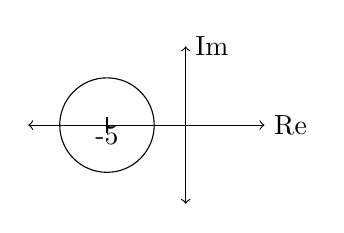
\begin{tikzpicture}[scale=0.2]
            \draw[<->] (-10, 0) -- (5, 0) node[right] {$\text{Re}$};
            \draw[<->] (0, -5) -- (0, 5) node[right] {$\text{Im}$};
            \draw (-5,-0.5) -- (-5,0.5) node[below] {-5};

            \draw{(-5, 0) circle [radius=3]};


        \end{tikzpicture}
    \end{center}


\end{examplebox}



\pagebreak

\section{Question 2: }
\subsection{Determine image of the line}
\begin{itemize}
    \item $f(z) = \frac{1}{z} \quad \{z \in \mathbb{C}: \text{Re}(z) = 2\}$ \hfill 2023 Q2(a), 2021 Q2(b)
    \item $f(z) = \frac{1}{z} \quad \{z \in \mathbb{C}: \text{Re}(z) = 1\}$ \hfill 2022 Q2(a), 2018 Q2(a), 2017 Q2(a)
\end{itemize}
\subsection{State and Use Cauchy-Riemann Equations}
\begin{itemize}
    \item State CRE, and use to prove $f(z) = \frac{1}{z}$ is holomoprhic on $\mathbb{C} \backslash \{0\}$ \hfill 2023 Q2(a)
    \item State CRE, and use to prove $f(z) = z^2$ is holomoprhic on $\mathbb{C}$ \hfill 2022 Q2(b)
    \item State CRE. Let $f = u+iv$ be holomoprhic on $\Omega \subset \mathbb{C}$. Prove $\nabla u$ and $\nabla v$ are perpendicular of equal length \hfill 2016 Q2(b)
\end{itemize}
\subsection{Show that}
\begin{itemize}
    \item If $\overline{f(z)} = f(\overline{z})$ for all $z \in \mathbb{C}$ then $f(x)$ is real for all $x \in \mathbb{R}$. And if in addition $f$ is holomoprhic at $x \in \mathbb{R}$ then $f'(x)$ is real. \hfill 2023 Q2(c)
    \item Define that is meant for a function $g$ to be harmonic. If $f = u +iv$ is holomoprhic on $\Omega \subset \mathbb{C}$, prove that $v(x,y)$ is a harmonic function, and that $\nabla u$ and $\nabla v$ are perpendicular of equal length. \hfill 2022 Q2(c), 2018 Q2(b)
    \item If $\overline{f(z)} = f(\overline{z})$ for all $z \in \mathbb{C}$ then $f(x)$ is real for all $x \in \mathbb{R}$. And if in addition $f$ is holomoprhic at $0$ then the function $f'(0)$ is real.\hfill 2021 Q2(a), 2017 Q2(c)
    \item Let $f(z) = u +iv$ be holomoprhic on an open subset $\Omega$ of the complex plane and let $h(u,v)$ be a harmonic function of $u$ and $v$ on $f(\Omega)$. Prove that $g(x,y) = h(u(x,y), v(x,y))$ is harmonic on $\Omega$ (You may assume $\nabla u, \nabla v$ are equal length and perpendicular)\hfill 2021 Q2(c)
    \item Define what is meant for a function $f(z)$ to be holomoprhic at a point $z_0 \in \mathbb{C}$ and prove that $f(z) = z^2$ is holomoprhic and find its derivative there. Hence prove that the product $uv$ is harmonic where $f=u +iv$ \hfill 2018 Q2(c)
    \item Define what is meant for a function $f(z)$ to be holomoprhic at a point $z_0 \in \mathbb{C}$ and prove that $f(z) = \frac{1}{z}$ is holomoprhic on $\mathbb{C} \backslash 0$ and find its derivative there (State any theorems used) \hfill 2017 Q2(b)
    \item Let $h(u,v)$ be a harmonic function of $u, v$ on $f(\Omega)$ (See 2016 Q2(b)). Prove that $g(x,y) = h(u(x,y), v(x,y))$ is harmonic on $\Omega$ \hfill 2016 Q2(c)
\end{itemize}
\subsection{Find Mobius Transformation}
\begin{itemize}
    \item $T(z) : (-1, 1, \infty) \mapsto (-1, -i, 1)$ \hfill 2023 Q2(d)
    \item $T(z) : (2, 1, -1) \mapsto (1, 0, \infty)$    \hfill 2022 Q2(d)
    \item $T(z) : (-i, -1, 1) \mapsto (1, 0, \infty)$ and find the inverse Mobius Transformation \hfill 2021 Q2(d)
    \item $T(z) : (-i, -1, i) \mapsto (1, 0, \infty)$ and find the inverse Mobius Transformation \hfill 2018 Q2(d), 2017 Q2(d)
    \item $T(z) : (-1, \frac{1}{2}, 2) \mapsto (1, 0, \infty)$ and find the inverse Mobius Transformation \hfill 2016 Q2(d)
\end{itemize}


\end{document}